\chapter{Introducción}
\section{Definición del Problema}   
Con la demanda incremental de aplicaciones, tanto para el entretenimiento 
como para el estudio biomédico, la información visual cada vez tiene un rol 
más importante. Sin embargo, la calidad de dicha información puede 
verse mermada con las etapas de adquisición, procesado, compresión, transmisión y reproducción.
Es por ello que poder evaluar dicha calidad se ha vuelto un 
tema cada vez más importante~\cite{RecentIQASurvey, IQABook, VisualMedicalQualityBook}.
Es por ello que, este Trabajo Fin de Grado (TFG) se centra en el estudio de la 
evaluación de la calidad de imágenes,
en inglés \emph{Image Quality assessment} (\emph{IQA})~\cite{MinkowskiFailure}.
Se trata de un problema fundamental en el procesamiento de imágenes y la visión 
por computador~\cite{CVAlgorithms,CVGeometry,CVModern,CVProcessing}, que hace referencia a la tarea de medir y cuantificar 
la calidad perceptual de una imagen, 
teniendo en cuenta factores como el contenido, la resolución, 
el contraste, las distorsiones visuales y la percepción humana. 
La mejora de estas técnicas suele estar altamente conectada con el avance 
en los estudios del sistema de visión humano~\cite{Wang2006ModernIQ}.
 
El problema de la evaluación de la calidad de la imagen se aborda mediante enfoques 
subjetivos y objetivos~\cite{Wang2006ModernIQ}.
\begin{itemize}
  \item Los enfoques subjetivos implican realizar experimentos 
perceptuales en los que se recopilan las opiniones y evaluaciones de los observadores 
humanos. Estos observadores pueden calificar las imágenes en términos de su 
calidad visual o realizar comparaciones entre diferentes versiones de una misma imagen. 
Con base a las respuestas recopiladas, se pueden establecer modelos y 
métricas que reflejen la calidad percibida por los humanos, también conocida
como \emph{mean opinion score, MOS}\footnote{
\emph{Mean Opinion Score} o valor medio de opinión, consiste en 
la media de la opinión de diversas personas para establecer un valor de referencia. 
}.
\item Los enfoques objetivos buscan desarrollar algoritmos y métricas 
que puedan estimar la calidad de la imagen sin intervención humana. 
Estos enfoques se basan en características y propiedades visuales extraídas automáticamente a partir de la 
imagen, que se utilizan para calcular una puntuación de calidad. Estas características 
pueden incluir medidas de nitidez, contraste, estructura, color, distribución de 
texturas y otros aspectos relevantes para la percepción visual.
\end{itemize}
 
La elección entre enfoques subjetivos u objetivos depende del contexto y los 
recursos disponibles. Los enfoques subjetivos son considerados como la referencia estándar 
para la evaluación de la calidad de la imagen, ya que capturan la apreciación 
humana. Sin embargo, estos enfoques pueden ser costosos y requieren de un número 
significativo de participantes. 
Por otro lado, los enfoques objetivos se pueden llegar a automatizar, haciendo que 
sean muy prácticos para grandes cantidades de datos y diversas aplicaciones.
 
No obstante, el objetivo del campo es desarrollar algoritmos y métricas que puedan proporcionar una 
estimación precisa y consistente de la calidad de la imagen, teniendo en cuenta
tanto aspectos subjetivos como objetivos respecto a las distorsiones~\cite{SJTU}.
Y, de esta forma, poder evaluar y comparar diferentes métodos de adquisición, compresión, 
restauración o manipulación de imágenes teniendo en cuenta que el receptor 
final es el humano.
 
Para abordar el problema de la IQA de forma objetiva, se emplean diversas técnicas y enfoques
\cite{MinkowskiFailure, Wang2006ModernIQ, VisualMedicalQualityBook}.
Entre ellos se incluyen métodos basados en características,
modelos de percepción visual, aprendizaje automático y técnicas de procesamiento de señales
\cite{SSIM, MMF, DSS}.
Uno de los enfoques más habituales consiste en utilizar características básicas de la imagen. 
Las características elementales de la imagen son por ejemplo el contraste, 
la nitidez, la exposición y la uniformidad del color~\cite{MinkowskiFailure,Wang2006ModernIQ}. 
Estas características pueden ser cuantificadas mediante algoritmos de procesamiento de 
imágenes y proporcionar una estimación inicial de la calidad. 
 
Por otro lado, los modelos de percepción visual intentan simular cómo el sistema 
visual humano percibe y evalúa la calidad de la imagen. Estos modelos se basan 
en el entendimiento de los mecanismos y procesos perceptuales del cerebro humano, 
y utilizan características visuales y estadísticas para calcular la calidad percibida
\cite{MinkowskiFailure, SSIM}.
Buscan emular la forma en que los humanos responden 
a las imágenes en términos de su calidad visual~\cite{VSI, CascadedIQA}.
 
Finalmente, se suelen emplear algoritmos de aprendizaje automático para tratar
de resolver el problema. Se intenta aproximar una función que a partir del conjunto 
de características extraídas pueda determinar la calidad de la imagen en una escala 
específica, generalmente en el rango de 0 a 10.

Entre las aplicaciones más comunes de los algoritmos de estimación de calidad se podrían citar las siguientes~\cite{VMAF, VMAFReproducibility, Applications}:  
la comparativa entre algoritmos de compresión (ya que permite elegir aquellos con 
menor pérdida de información), la generación de mapas de calidad\footnote{
  Nivel de calidad perceptual de diferentes regiones o píxeles de la imagen.
}
(permitiendo el estudio de métodos de reducción de ruido local)
y la determinación de la calidad del servicio de transmisión o \emph{quality-of-service (QoS)}
(ya que permiten evaluar los errores de transmisión). Se podría incluso 
extender al pre-procesamiento de datos de entrenamiento o estimar la precisión 
de un modelo de predicción basado en la calidad de los datos~\cite{ApplicationsOfIQA}.

El uso de algoritmos IQA se encuentra ampliamente difundido en el ámbito general de las imágenes 2D. 
Sin embargo, el número de métodos propuestos decrece al desplazarnos a tres dimensiones.
Además, en el ámbito médico, la naturaleza de estas imágenes y las distorsiones que pueden 
presentar (véase Figura \ref{fig:DicomDistortionsExample}) implican una disminución en 
la precisión de los modelos cuando se aplican directamente sobre ellas~\cite{VisualMedicalQualityBook}.

\begin{figure}[htp]
  \centering 
  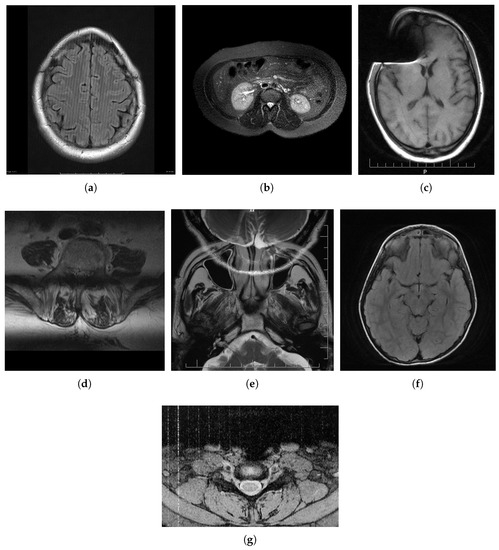
\includegraphics[width=.7\textwidth]{imagenes/chapter2/MedicalDistortions}
  \caption[Ejemplo de artefactos sobre imágenes DICOM.]{Ejemplo de artefactos sobre imágenes médicas~\cite{MoreMedicalDistortion}: 
     (a) \emph{herringbone}, (b) \emph{ghosting}, (c) susceptibilidad magnética, (d) superposición de cortes, (e) \emph{aliasing}, (f) efecto de Gibbs, y (g) \emph{zipper}.
   }
  \label{fig:DicomDistortionsExample}
\end{figure}

En la Figura \ref{fig:DicomDistortionsExample} se aprecian las siguientes distorsiones:
\begin{description}
  \item[(a)] \textbf{\emph{Herringbone}}: causa variaciones en intensidad y superposición 
    de bandas oscuras en imágenes debido a la transformada de Fourier.
  \item[(b)] \textbf{\emph{Ghosting}}: influenciado por reacciones físicas del paciente, 
    factores ambientales y movimientos pulsátiles, como latidos cardíacos, 
    puede causar distorsiones que se superponen con la imagen.
  \item[(c)] \textbf{Susceptibilidad magnética}: al ubicar tejidos en un campo magnético, 
    su magnetización desigual debido a la susceptibilidad magnética causa 
    distorsiones geométricas y variaciones de señal, acentuadas por implantes 
    metálicos altamente susceptibles.
  \item[(d)] \textbf{Superposición de cortes}: pérdida de señal visible en la imagen 
    debido a la adquisición desde múltiples ángulos. 
    En esta distorsión, las secciones en los bordes tienen una intensidad de señal 
    reducida y no crean un perfil de corte con bordes rectos.
  \item[(e)] \textbf{\emph{Aliasing}}: Los artefactos de aliasing surgen cuando el campo 
    de visión es menor que la zona corporal capturada, generando superposición 
    de estructuras regulares. En imágenes médicas, estas distorsiones pueden 
    aparecer como un patrón de franjas o líneas que no corresponden 
    correctamente a la anatomía real.
  \item[(f)] \textbf{Efecto de Gibbs}: también conocidos como artefactos de truncamiento 
    o artefactos de anillos, son una serie de líneas en la imagen de resonancia 
    magnética que aparecen paralelas al área donde ha ocurrido un cambio repentino 
    e intenso en la intensidad de la señal.
  \item[(g)] \textbf{\emph{Zipper}}: área de píxeles alternantes claros y oscuros, presente en la dirección de codificación de frecuencia y que aparece en toda la serie de imágenes.
\end{description}
La mayoría de estas distorsiones, y combinaciones de ellas, no ocurren de forma natural 
en las imágenes habituales del problema IQA. 
Como consecuencia, es necesario diseñar adaptaciones de los modelos actuales y, por lo tanto, el número de métodos médicos 
existentes se reduce, con ninguno, al momento de escritura, aplicado directamente a la reconstrucción 3D. 
Dichas reconstrucciones suelen ser nubes de puntos~\cite{WhyUsePointCloud} y las distorsiones 
anteriores afectan al resultado final. 

Las nubes de puntos o conjunto de puntos arbitrarios extraídos de la superficie 
de un objeto de interés es una de las representaciones más comunes y flexibles:
los objetos representados ya sea mediante volúmenes de vóxeles o mallas poligonales
pueden muestrearse fácilmente en nubes de puntos. Además, la adquisición de 
datos a través de escaneo, segmentación u obtenidos de algoritmos de reconstrucción 
3D generalmente proporcionan información geométrica en forma de un conjunto de puntos. 
Las superficies reconstruidas pueden ser aplicadas para:
medición morfológica del grosor de la corteza o los huesos,
extracción de la línea central (esqueleto de curva) para traqueotomía o colonoscopía,
particionamiento de superficies para clasificación de superficies corticales o
anatómicas, así como registro y correspondencia de formas de tumores o huesos carpales 
\cite{WhyUsePointCloud}.

Es por ello que se propone investigar específicamente el uso de métodos tridimensionales
para el ámbito biomédico, aplicado a las reconstrucciones y visualizaciones volumétricas 
que se suelen emplear en medicina. El proyecto esta disponible en \url{https://github.com/CodeBoy-source/TFG_NRPCQA}.

\section{Motivación}
 
En el caso del ámbito biomédico, dados los rápidos avances 
de las técnicas no invasivas y la gran cantidad de fabricantes 
de equipamientos, nació el estándar \emph{DICOM}~\cite{Parisot1995} en 1995 
con el objeto de hacer que el intercambio de imágenes médicas se realizase de forma 
fácil, segura y con alta calidad. Este estándar pretendía permitir la integración con diversos sistemas, 
almacenar información extra en forma de metadatos y anotaciones, así como segmentaciones que facilitasen la reconstrucción 3D de diferentes regiones anatómicas.

Cada vez más frecuentemente se emplean volúmenes tridimensionales, como tomografías computarizadas o
resonancias magnéticas en lugar de radiografías convencionales, porque 
proporcionan una visión más completa y detallada de la anatomía y las estructuras 
internas del cuerpo (véase Figura \ref{fig:SlicerVisualization}). 
Esta visualización tridimensional permite a los médicos y personal sanitario 
identificar con mayor precisión lesiones, enfermedades o anormalidades,
así como facilitar la planificación quirúrgica, entre otros~\cite{3DImagingInMedicine, 3DImagingInMedicine2, ADAS3D}.
 
\begin{figure}[htp]
  \begin{center}
    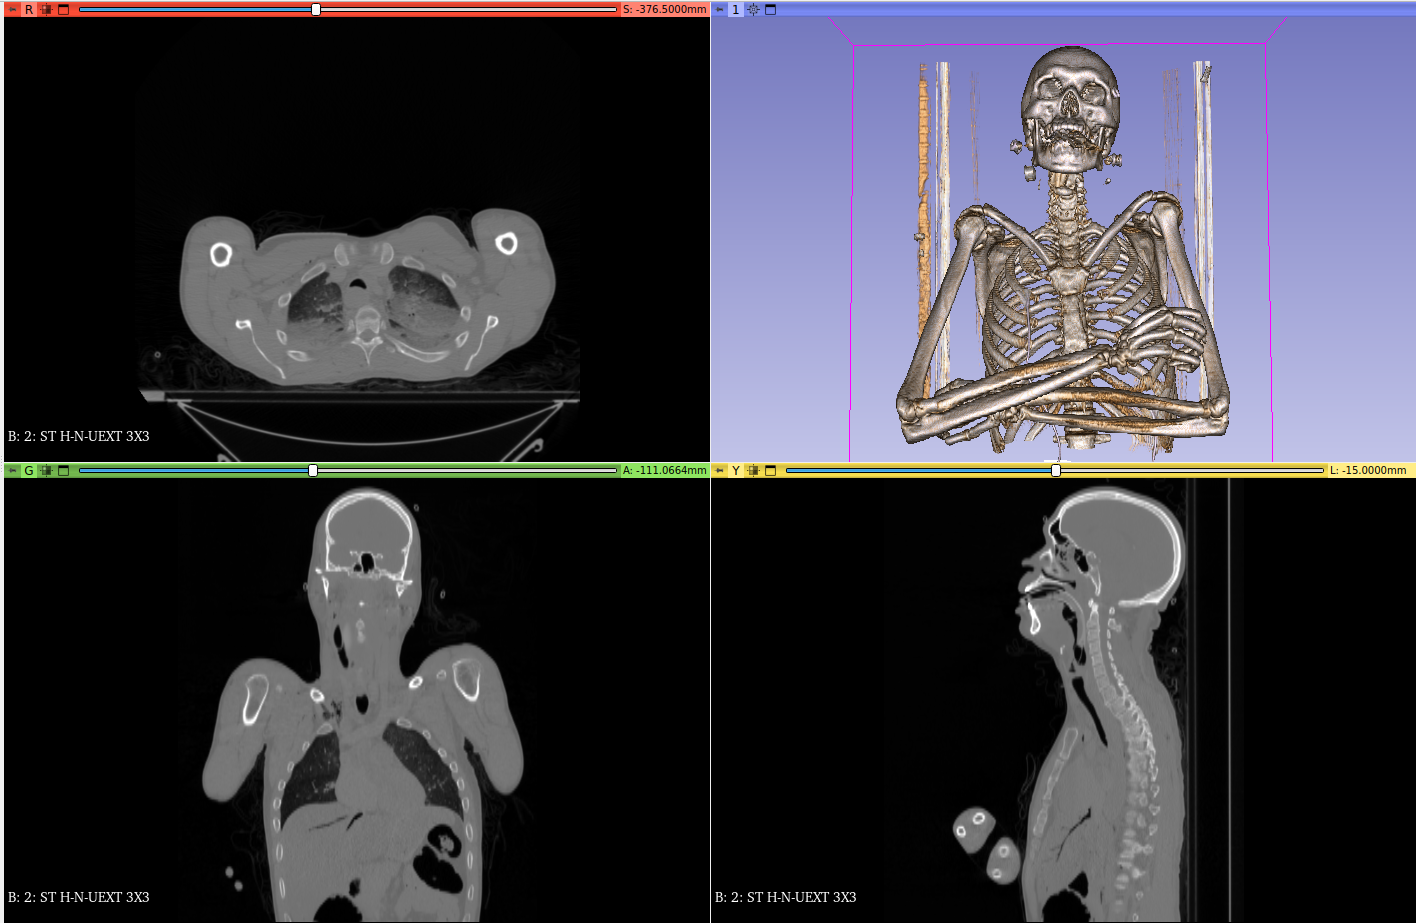
\includegraphics[width=0.8\textwidth]{imagenes/chapter1/SlicerVisualization}
  \end{center}
  \caption[Ejemplo de visualización de un directorio DICOM.]{Ejemplo de visualización de un directorio \emph{DICOM}
    empleando \emph{Slicer3D}~\cite{Slicer3D}. Se pueden observar
  las proyecciones axial (arriba izquierda), coronal (abajo izquierda),
  y sagital (abajo derecha). También se muestra una renderización volumétrica
de los huesos (arriba derecha).
} 
  \label{fig:SlicerVisualization}
\end{figure}

No obstante, cabe mencionar que las distorsiones
están muy presentes en las imágenes médicas~\cite{MedicalImpactOfDistortions}.
Estas, a su vez, podrían afectar al volumen 3D que se puede generar a partir 
las imágenes médicas, influyendo en el análisis y diagnóstico asociados. Por ejemplo, 
 en~\cite{XrayRejectionFactor} se estudiaron las razones por las que se suelen 
rechazar las radiografías y su relación relación con el diagnóstico final. 
Reveló que la mayoría de los rechazos se producen por 
errores de posicionamiento, valores inadecuados de exposición, artefactos 
y los problemas de cooperación del paciente. 
Además, no es difícil imaginar que una alta 
calidad de imagen médica tiene implicaciones significativas sobre el cuidado
del paciente. Ya que la mala calidad de imagen puede provocar diagnósticos erróneos. 
Sin mencionar los elevados costes que supone realizar 
nuevas pruebas para conciliar las anteriores. 

Por todo ello, las contribuciones relativas al IQA en el 
ámbito biomédico son claramente bienvenidas, resultando en 
una potencial reducción de costes (menos pruebas), de tiempo de consulta, y mejora 
en la calidad del diagnóstico médico. 

\section{Objetivos}
El objetivo principal de este Trabajo de Fin de Grado (TFG) 
consiste en desarrollar un \textbf{método adecuado para abordar al 
problema de la estimación de la calidad de imágenes médicas tridimensionales}. 
Este objetivo se puede descomponer en una serie de metas parciales: 
\begin{enumerate}
  \item Realizar una revisión exhaustiva del estado del arte para la estimación de calidad 
    de imágenes 3D, así como de la calidad de imágenes médicas 3D en particular.
  \item Estudiar las distorsiones de imagen más comunes, en general, y analizar los patrones de distorsión que afectan la calidad de las imágenes 
    biomédicas.
  \item Analizar pausadamente los enfoques de inteligencia artificial más prometedores que permitan abordar el problema planteado. 
  \item Generar un conjunto de datos sintético que permita validar 
    los métodos empleados. Para ello, será necesario estudiar diferentes 
    estrategias y métricas de evaluación objetivas.
  \item Realizar un estudio experimental que permita validar los enfoques 
    propuestos y extraer conclusiones sobre su aplicabilidad al problema. 
\end{enumerate}

\begin{figure}
  \begin{center}
    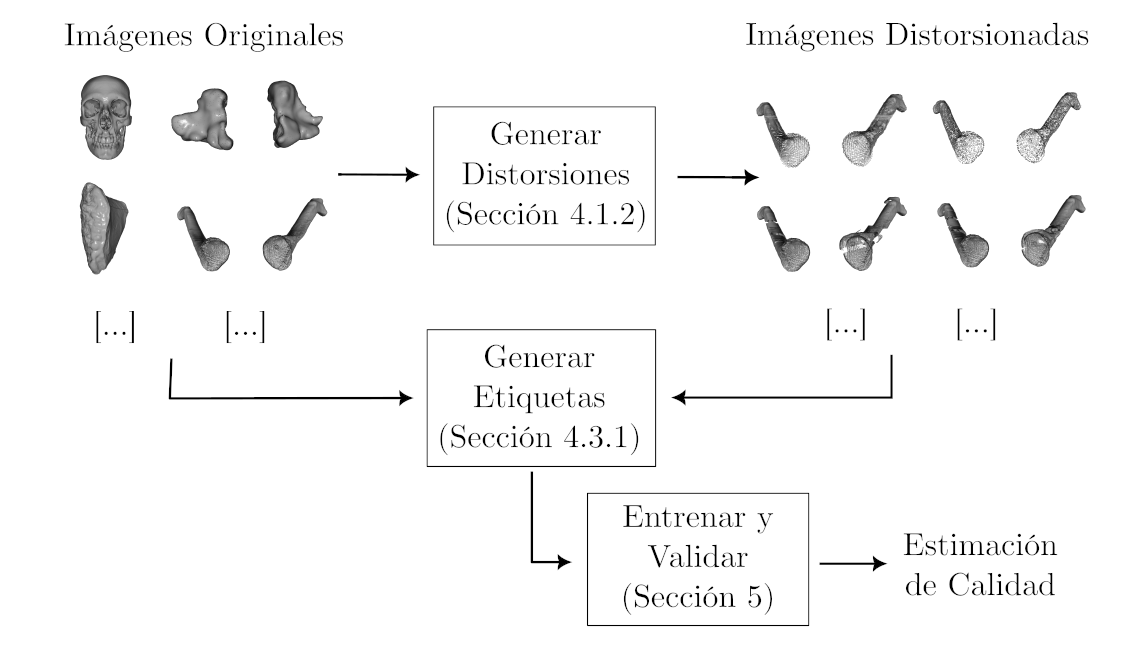
\includegraphics[width=\textwidth]{imagenes/chapter1/Objetivos}
  \end{center}
  \caption{Objetivos de este proyecto.}
  \label{fig:Objetivos}
\end{figure}


\section{Planificación del proyecto}
Al planificar el proyecto, es fundamental tener en cuenta que el TFG 
tiene una carga de 12 créditos ECTS, donde cada 
crédito representa aproximadamente 25 horas de trabajo. 
En total, se estima que se necesitarán alrededor de 300 horas para llevar a cabo 
el proyecto. Considerando que el segundo cuatrimestre tiene aproximadamente 20 semanas, 
se requerirá dedicar al TFG unas 15 horas por semana, lo cual equivaldría a unas 3 horas 
diarias durante 5 días a la semana.
 
La naturaleza del proyecto no presenta una complejidad significativa en términos 
de su alcance y requisitos, y el equipo de trabajo tampoco incluye un numeroso grupo 
de personas cuya colaboración deba ser sincronizada, lo cual permite abordar su desarrollo a través de un 
enfoque de ciclo de vida en cascada~\cite{ModeloEnCascada}. 
No obstante, bajo este enfoque se evita retroceder en cualquiera de las fases 
del ciclo, y aunque se espera que el diseño y los requisitos del sistema sean 
estables, existe la posibilidad de realizar ajustes menores conforme se obtenga
más información sobre el problema y los métodos. 
Es por ello que utilizamos una pequeña variante, la versión con retroalimentación.
 
Las fases del ciclo de vida son: 
\begin{itemize}
  \item Análisis de requisitos: Consiste en reuniones iniciales con los clientes, 
    en este caso sería los directores del TFG. Se organiza el análisis bibliográfico 
    del problema \emph{IQA} y \emph{PCQA}\footnotemark[4], teniendo en cuenta un estudio previo 
    de las distorsiones médicas.
  \item Diseño: Consiste en la investigación y selección de métodos conforme 
    al análisis anterior, tanto para la resolución como la validación de la solución. 
    Así como pruebas preliminares y diseño del software de experimentación. 
  \item Implementación: Consiste en la adaptación de las técnicas encontradas, 
    implementación de nuevas funcionalidades y generación de un conjunto de datos 
    médicos.
  \item Pruebas: Realización de diversos experimentos de validación, tanto al 
    la generación de las distorsiones como a los modelos y resultados.
\end{itemize}
\footnotetext[4]{\emph{Point cloud quality assessment} o estimación de calidad 
de nubes de puntos} 
\begin{table}[htp]
\centering
\resizebox{\textwidth}{!}{%
\begin{tabular}{|c|c|ll|llll|llll|lllll|llll|llll|}
\hline
\rowcolor[HTML]{FFC702} 
\cellcolor[HTML]{FFC702} & \cellcolor[HTML]{FFC702} & \multicolumn{2}{c|}{\cellcolor[HTML]{FFC702}\textbf{Febrero}} & \multicolumn{4}{c|}{\cellcolor[HTML]{FFC702}\textbf{Marzo}} & \multicolumn{4}{c|}{\cellcolor[HTML]{FFC702}\textbf{Abril}} & \multicolumn{5}{c|}{\cellcolor[HTML]{FFC702}\textbf{Mayo}} & \multicolumn{4}{c|}{\cellcolor[HTML]{FFC702}\textbf{Junio}} & \multicolumn{4}{c|}{\cellcolor[HTML]{FFC702}\textbf{Julio}} \\ \cline{3-25} 
\rowcolor[HTML]{FFC702} 
\multirow{-2}{*}{\cellcolor[HTML]{FFC702}\textbf{Tarea}} & \multirow{-2}{*}{\cellcolor[HTML]{FFC702}\begin{tabular}[c]{@{}c@{}}\textbf{Semanas -}\\ \textbf{Horas}\end{tabular}} & \multicolumn{1}{c}{\cellcolor[HTML]{FFC702}21} & \multicolumn{1}{c|}{\cellcolor[HTML]{FFC702}28} & \multicolumn{1}{c}{\cellcolor[HTML]{FFC702}07} & \multicolumn{1}{c}{\cellcolor[HTML]{FFC702}14} & \multicolumn{1}{c}{\cellcolor[HTML]{FFC702}21} & \multicolumn{1}{c|}{\cellcolor[HTML]{FFC702}28} & \multicolumn{1}{c}{\cellcolor[HTML]{FFC702}04} & \multicolumn{1}{c}{\cellcolor[HTML]{FFC702}11} & \multicolumn{1}{c}{\cellcolor[HTML]{FFC702}18} & \multicolumn{1}{c|}{\cellcolor[HTML]{FFC702}25} & \multicolumn{1}{c}{\cellcolor[HTML]{FFC702}02} & \multicolumn{1}{c}{\cellcolor[HTML]{FFC702}09} & \multicolumn{1}{c}{\cellcolor[HTML]{FFC702}16} & \multicolumn{1}{c}{\cellcolor[HTML]{FFC702}23} & \multicolumn{1}{c|}{\cellcolor[HTML]{FFC702}30} & \multicolumn{1}{c}{\cellcolor[HTML]{FFC702}06} & \multicolumn{1}{c}{\cellcolor[HTML]{FFC702}13} & \multicolumn{1}{c}{\cellcolor[HTML]{FFC702}20} & \multicolumn{1}{c|}{\cellcolor[HTML]{FFC702}27} & \multicolumn{1}{c}{\cellcolor[HTML]{FFC702}04} & \multicolumn{1}{c}{\cellcolor[HTML]{FFC702}11} & \multicolumn{1}{c}{\cellcolor[HTML]{FFC702}18} & \multicolumn{1}{c|}{\cellcolor[HTML]{FFC702}25} \\ \hline
Análisis de Requisitos & 4 - 60 & \cellcolor[HTML]{9B9B9B} & \cellcolor[HTML]{9B9B9B} & \cellcolor[HTML]{9B9B9B} & \cellcolor[HTML]{9B9B9B} & \cellcolor[HTML]{9B9B9B} &  &  &  &  &  &  &  &  &  &  &  &  &  &  &  &  &  &  \\ \cline{1-1}
Diseño & 4 - 60 &  &  &  &  & & \cellcolor[HTML]{9B9B9B} & \cellcolor[HTML]{9B9B9B} & \cellcolor[HTML]{9B9B9B} & \cellcolor[HTML]{9B9B9B}  & \cellcolor[HTML]{9B9B9B} &  &  &  &  &  &  &  &  &  &  &  &  &  \\ \cline{1-1}
Implementación & 6 - 90 &  &  &  &  &  &  &  &  & & & \cellcolor[HTML]{9B9B9B} & \cellcolor[HTML]{9B9B9B} & \cellcolor[HTML]{9B9B9B} & \cellcolor[HTML]{9B9B9B} & \cellcolor[HTML]{9B9B9B} &  &  &  &  &  &  &  &  \\ \cline{1-1}
Pruebas & 6 - 90 &  &  &  &  &  &  &  &  &  &  &  &  &  &  & & \cellcolor[HTML]{9B9B9B} & \cellcolor[HTML]{9B9B9B} & \cellcolor[HTML]{9B9B9B} & \cellcolor[HTML]{9B9B9B} & &  &  &  \\ \hline
\end{tabular}%
}
\caption{Planificación temporal inicial del proyecto.}
\label{tab:PlanificacionTemporal}
\end{table}

La planificación inicial se muestra en la Tabla \ref{tab:PlanificacionTemporal}. 
Dicha planificación sufrió ciertos retrasos debido a que el alumno estaba realizando prácticas de empresa, tenía 
una asignatura y participaba de un curso de \emph{Google} ofrecido por la universidad.
Además, se esperaba que ocurrieran retrasos, sobre todo en la implementación, 
como se puede ver en la Tabla \ref{tab:PlanificacionFinal}, dada la novedad de la propuesta
y la dificultad del problema. En concreto, por ejemplo, el hecho de simular las distorsiones 
médicas fue un proceso iterativo y manual que llevó más tiempo de lo esperado. 

\begin{table}[H]
\resizebox{\textwidth}{!}{%
\begin{tabular}{|c|c|ll|llll|llll|lllll|llll|llll|}
\hline
\rowcolor[HTML]{FFC702} 
\cellcolor[HTML]{FFC702} & \cellcolor[HTML]{FFC702} & \multicolumn{2}{c|}{\cellcolor[HTML]{FFC702}\textbf{Febrero}} & \multicolumn{4}{c|}{\cellcolor[HTML]{FFC702}\textbf{Marzo}} & \multicolumn{4}{c|}{\cellcolor[HTML]{FFC702}\textbf{Abril}} & \multicolumn{5}{c|}{\cellcolor[HTML]{FFC702}\textbf{Mayo}} & \multicolumn{4}{c|}{\cellcolor[HTML]{FFC702}\textbf{Junio}} & \multicolumn{4}{c|}{\cellcolor[HTML]{FFC702}\textbf{Julio}} \\ \cline{3-25} 
\rowcolor[HTML]{FFC702} 
\multirow{-2}{*}{\cellcolor[HTML]{FFC702}\textbf{Tarea}} & \multirow{-2}{*}{\cellcolor[HTML]{FFC702}\begin{tabular}[c]{@{}c@{}}\textbf{Semanas -}\\ \textbf{Horas}\end{tabular}} & \multicolumn{1}{c}{\cellcolor[HTML]{FFC702}21} & \multicolumn{1}{c|}{\cellcolor[HTML]{FFC702}28} & \multicolumn{1}{c}{\cellcolor[HTML]{FFC702}07} & \multicolumn{1}{c}{\cellcolor[HTML]{FFC702}14} & \multicolumn{1}{c}{\cellcolor[HTML]{FFC702}21} & \multicolumn{1}{c|}{\cellcolor[HTML]{FFC702}28} & \multicolumn{1}{c}{\cellcolor[HTML]{FFC702}04} & \multicolumn{1}{c}{\cellcolor[HTML]{FFC702}11} & \multicolumn{1}{c}{\cellcolor[HTML]{FFC702}18} & \multicolumn{1}{c|}{\cellcolor[HTML]{FFC702}25} & \multicolumn{1}{c}{\cellcolor[HTML]{FFC702}02} & \multicolumn{1}{c}{\cellcolor[HTML]{FFC702}09} & \multicolumn{1}{c}{\cellcolor[HTML]{FFC702}16} & \multicolumn{1}{c}{\cellcolor[HTML]{FFC702}23} & \multicolumn{1}{c|}{\cellcolor[HTML]{FFC702}30} & \multicolumn{1}{c}{\cellcolor[HTML]{FFC702}06} & \multicolumn{1}{c}{\cellcolor[HTML]{FFC702}13} & \multicolumn{1}{c}{\cellcolor[HTML]{FFC702}20} & \multicolumn{1}{c|}{\cellcolor[HTML]{FFC702}27} & \multicolumn{1}{c}{\cellcolor[HTML]{FFC702}04} & \multicolumn{1}{c}{\cellcolor[HTML]{FFC702}11} & \multicolumn{1}{c}{\cellcolor[HTML]{FFC702}18} & \multicolumn{1}{c|}{\cellcolor[HTML]{FFC702}25} \\ \hline
Análisis de Requisitos & 5 - 75 & \cellcolor[HTML]{9B9B9B} & \cellcolor[HTML]{9B9B9B} & \cellcolor[HTML]{9B9B9B} & \cellcolor[HTML]{9B9B9B} & &  &  &  &  &  &  &  &  &  &  &  &  &  &  &  &  &  &  \\ \cline{1-1}
Diseño & 4 - 60 &  &  &  &  & \cellcolor[HTML]{9B9B9B} & \cellcolor[HTML]{9B9B9B} & \cellcolor[HTML]{9B9B9B} & \cellcolor[HTML]{9B9B9B} & &  &  &  &  &  &  &  &  &  &  &  &  &  &  \\ \cline{1-1}
Implementación & 8 - 120 &  &  &  &  &  &  &  &  &  \cellcolor[HTML]{9B9B9B} & \cellcolor[HTML]{9B9B9B} & \cellcolor[HTML]{9B9B9B} & \cellcolor[HTML]{9B9B9B} & &  & \cellcolor[HTML]{9B9B9B}  & \cellcolor[HTML]{9B9B9B}  & & & \cellcolor[HTML]{9B9B9B} & \cellcolor[HTML]{9B9B9B} &  &  &  \\ \cline{1-1}
Pruebas & 6 - 90 &  &  &  &  &  &  &  &  &  &  &  &  & \cellcolor[HTML]{9B9B9B}   & \cellcolor[HTML]{9B9B9B} & & & \cellcolor[HTML]{9B9B9B} & \cellcolor[HTML]{9B9B9B} &  &  & \cellcolor[HTML]{9B9B9B} & \cellcolor[HTML]{9B9B9B} & \\ \hline
\end{tabular}%
}
\caption{Planificación resultante del proyecto.}
\label{tab:PlanificacionFinal}
\end{table}

Para realizar este proyecto se tuvo en cuenta los siguientes materiales:
suscripción a \emph{Google Colab Pro}, un portátil personal de gama media, 
\emph{Google Drive 100GB} y otros gastos. 
Además, para el coste estimado, se asume un salario de 25\officialeuro/hora, como para un investigador \emph{senior} o
responsable I+D de una empresa tecnológica en España. 
 
Respecto al servidor GPU, con las especificaciones actuales de \emph{Google}, 
se estima un coste aproximado de 10.000\officialeuro. Se asume una amortización de 2 años, 
lo que implica un pago diario de 13.70\officialeuro. El desglose total de los costes 
se puede ver en la siguiente Tabla \ref{tab:TotalGastos}.

\begin{table}[H]
\centering
\begin{tabular}{ll}
\hline
\multicolumn{1}{|l|}{\cellcolor[HTML]{FFCB2F}{\textbf{Fecha inicio}}} & \multicolumn{1}{l|}{21/02/2022} \\ \hline
\multicolumn{1}{|l|}{\cellcolor[HTML]{FFCB2F}{\textbf{Fecha fin}}} & \multicolumn{1}{l|}{25/07/2022} \\ \hline
\multicolumn{1}{|l|}{\cellcolor[HTML]{FFCB2F}{\textbf{Duración}}} & \multicolumn{1}{l|}{154 días, 110 laborables} \\ \hline
\textbf{} & 
\end{tabular}
\caption{Total de horas y días trabajados.}
\label{tab:TotalTrabajado}
\end{table}

\begin{table}[H] 
  \centering
  \begin{tabular}{ll}
\hline
\rowcolor[HTML]{FFCB2F} 
\multicolumn{1}{|c|}{\cellcolor[HTML]{FFCB2F}{\textbf{Item}}} & \multicolumn{1}{c|}{\cellcolor[HTML]{FFCB2F}{\textbf{Costo}}} \\ \hline
\multicolumn{1}{|l|}{Salario} & \multicolumn{1}{l|}{8 250.00\officialeuro} \\ \hline
\multicolumn{1}{|l|}{Portátil de Gama Media} & \multicolumn{1}{l|}{700.00\officialeuro} \\ \hline
\multicolumn{1}{|l|}{Google Colab Pro} & \multicolumn{1}{l|}{55.50\officialeuro} \\ \hline
\multicolumn{1}{|l|}{Servidor GPU} & \multicolumn{1}{l|}{2 109.8\officialeuro} \\ \hline
\multicolumn{1}{|l|}{Google Drive 100GB} & \multicolumn{1}{l|}{10.00\officialeuro} \\ \hline
\multicolumn{1}{|l|}{Otros} & \multicolumn{1}{l|}{300.00\officialeuro} \\ \hline
\multicolumn{1}{|r|}{\cellcolor[HTML]{FFCB2F}{\textbf{Total}}} & \multicolumn{1}{l|}{ 11.425,3 \officialeuro} \\ \hline
\textbf{} & 
\end{tabular}
\caption{Estimación final de coste del proyecto.}
\label{tab:TotalGastos}
\end{table}
